\chapter{Resultados e Discussão}
\label{cap:resultados}

Este capítulo apresenta a avaliação experimental da arquitetura descrita no
Capítulo~\ref{cap:proposta}. Os resultados aqui relatados são os mesmos que
sustentam o artigo publicado no periódico \textit{IEEE Access}, aceito em novembro
de 2026, e foram obtidos integralmente em simulação, no ambiente descrito na
Seção~\ref{sec:setup-ambiente}.

Antes de qualquer número, convém fixar o que esta avaliação pode e o que não pode
sustentar. A percepção é abstraída em eventos-oráculo: o simulador publica
modalidade, intensidade e posição de cada evento sem incerteza associada, e a
transformada de localização é fixa. Em consequência, os resultados falam da
\emph{lógica de decisão} da arquitetura --- quando desviar, de que se afastar, o que
inspecionar primeiro --- e não de um sistema pronto para implantação. A
Seção~\ref{sec:res-ruido} relaxa parcialmente a primeira dessas idealizações
injetando ruído na percepção, e a Seção~\ref{sec:res-ameacas} enumera o que
permanece fora do alcance do estudo.

\section{Protocolo de Análise}
\label{sec:res-protocolo}

Relatam-se os valores finais, por execução, de cada métrica, agregados sobre até
$n=10$ execuções por configuração. Vários desfechos são contagens limitadas, com
variância nula ou quase nula, para as quais as premissas de um teste $t$ paramétrico
não se sustentam. As comparações entre grupos empregam, portanto, testes livres de
distribuição: o $U$ de Mann--Whitney, cujo $p$ é calculado caso a caso --- a
distribuição \emph{exata} de $U$ para amostras sem empates com $n_1+n_2\le20$
(todos os pares aqui), o $p$ exato de permutação bilateral para braços constantes
completamente separados, e a aproximação normal corrigida para empates apenas quando
há empates. Cada comparação é acompanhada do tamanho de efeito $\delta$ de Cliff e de
intervalos de confiança \textit{bootstrap} de $95\%$. Equivalência, quando
mencionada, é avaliada por dois testes unilaterais (TOST); taxas de sucesso por
missão são relatadas com intervalos de Wilson.

\subsection{Execuções Válidas e Confiabilidade de Inicialização}

Execuções em que a plataforma não se moveu (distância percorrida $\approx 0$)
constituem um desfecho de confiabilidade de inicialização, não um resultado de
navegação. Das $160$ execuções tentadas, $154$ atenderam ao critério de movimento
para análise comportamental e $6$ permaneceram imóveis. O critério observável e
publicado para essas seis é a \emph{imobilidade} --- o critério de distância do
analisador; a maioria acumula relógio de missão sem qualquer deslocamento. Lemos
esse padrão como consistente com uma falha de \emph{inicialização} (o contêiner de
navegação não subindo o robô), mas não certificamos essa causa de infraestrutura a
partir dos \textit{logs} brutos publicados.

Relatam-se duas visões complementares, em vez de agregá-las:

\begin{enumerate}
    \item desempenho \emph{condicional à inicialização bem-sucedida}, calculado
    sobre as execuções válidas ($n=8$ a $10$ por configuração);
    \item confiabilidade de partida \emph{por tentativa} ($154/160 = 96{,}25\%$).
\end{enumerate}

As execuções imóveis \emph{não} são promediadas nas métricas comportamentais --- sua
distância nula e inspeção nula enviesariam médias e taxas --- e são relatadas
separadamente como desfecho de confiabilidade. Os valores por execução, com
sementes e desfechos individuais, são publicados junto ao código.

\subsection{Alegações Primárias e Exploratórias}
\label{sec:res-familias}

A fronteira entre alegações confirmatórias e exploratórias é fixada aqui e marcada
em cada afirmação, e não apenas nas tabelas. É preciso ser exato quanto a que parte
da família foi fixada antecipadamente.

Os três \emph{contrastes} foram especificados antes de a nova bateria gravar seu
primeiro arquivo de resultado: a camada proposta contra a heurística genérica e
contra a variante de seleção de um fator, no cenário \texttt{default}; e a ablação
somente-\textit{keep-out} contra a patrulha fixa portando o mesmo \textit{keep-out}
(KOa \textit{vs.} KOF), no risco sobre a rota. O que o registro estabelece é
exatamente isso: o plano de análise publicado carrega os três contrastes em um
\textit{commit} que precede a primeira execução arquivada em cerca de uma hora. Não
se alega mais do que a ordenação que esse \textit{commit} demonstra.

O \emph{conjunto de desfechos} sobre os quais cada contraste é avaliado \emph{não}
foi declarado antecipadamente: os cinco aqui relatados --- anomalias inspecionadas,
distância mínima ao risco, duração da missão, recuos e tempo de investigação ---
foram fixados após as execuções. Chamamos esses quinze testes de \emph{família de
comparação primária com desfechos especificados retrospectivamente}, e não de
família confirmatória: a correção de Holm trata a multiplicidade \emph{dentro da
família tal como relatada}, mas não torna prospectiva a escolha dos desfechos, e
registro público é questão distinta, que tampouco se alega. O conjunto completo é
tabulado sem omissão de teste, de modo que o denominador possa ser conferido em vez
de aceito por confiança.

Todo o restante --- os cenários \texttt{conflict} e \texttt{adverse}, as varreduras
de limiar e de histerese, a configuração de risco marginal e toda reanálise de
execuções previamente gravadas --- é \emph{exploratório}, é relatado com $p$ não
corrigido e é rotulado como exploratório na própria frase que o enuncia.

\section{Detecção e Comportamento de Inspeção}
\label{sec:res-inspecao}

O resultado central é que a camada reativa converte uma patrulha de cobertura em um
comportamento de inspeção. A Tabela~\ref{tab:res-principal} consolida as métricas
por configuração.

A linha de base fixa (E1) inspeciona \emph{nenhuma} anomalia: percorre a ronda e
nunca se desvia ($0{,}0\pm0{,}0$). Com a camada \textsc{Stay Alert}, o robô
inspeciona \emph{todas as três} anomalias em toda execução válida do cenário padrão,
em qualquer ajuste de $\eta$, inclusive na ablação $\eta=0$ (E0--E4 todas em
$3{,}0\pm0{,}0$; $\delta$ de Cliff igual a $1$, permutação exata
$p=1{,}1\times10^{-5}$ contra E1). Essa completude se degrada sob ruído alto de
percepção (Seção~\ref{sec:res-ruido}) e sob aglomeração densa
(Seção~\ref{sec:res-adverso}), ambas quantificadas adiante.

Convém registrar que a linha de base de campo potencial artificial (APF) também
inspeciona as três ($3{,}0\pm0{,}0$), o que confirma que um esquema reativo de
simplicidade comparável produz a resposta à anomalia. A diferença entre os métodos
está em eficiência e segurança, discutidas adiante, e não na contagem bruta de
inspeções. A Figura~\ref{fig:res-traj} mostra o mecanismo: a camada reativa deixa a
patrulha para alcançar a pose de parada de cada anomalia e retorna, ao passo que E1
traça a ronda diretamente.

\begin{table}[htb]
\centering
\caption{Resultados por configuração (média\,$\pm$\,desvio padrão sobre execuções
válidas). E1 é a patrulha fixa de referência; E0 é a ablação com \textsc{Stay Alert}
ativa e peso de atualização de valor $\eta=0$; E2--E4 ativam \textsc{Stay Alert} com
$\eta\in\{0{,}3;\,0{,}5;\,0{,}8\}$; E5 é o cenário adverso ($\eta=0{,}5$); APF é a
linha de base de campo potencial artificial. O total de anomalias do cenário é $3$
(E0--E4, APF) e $5$ (E5). O ``resíduo de atualização'' é
$|\alpha\delta+\eta\Phi|$ completo, identicamente nulo quando a atualização de valor
está inativa (E1, APF). O APF, sendo um controlador contínuo de forças, não possui
contagem discreta de desvios de rota.}
\label{tab:res-principal}
\footnotesize
\setlength{\tabcolsep}{4pt}
\begin{tabular}{lccccccc}
\hline
\textbf{Métrica} & \textbf{E1} & \textbf{E0 ($\eta{=}0$)} & \textbf{E2} & \textbf{E3} & \textbf{E4} & \textbf{E5} & \textbf{APF}\\
\hline
Anomalias inspecionadas    & $0{,}0\pm0{,}0$ & $3{,}0\pm0{,}0$ & $3{,}0\pm0{,}0$ & $3{,}0\pm0{,}0$ & $3{,}0\pm0{,}0$ & $4{,}9\pm0{,}3$ & $3{,}0\pm0{,}0$\\
Desvios de rota            & $0{,}0\pm0{,}0$ & $4{,}0\pm0{,}0$ & $4{,}0\pm0{,}0$ & $4{,}0\pm0{,}0$ & $4{,}0\pm0{,}0$ & $9{,}4\pm0{,}8$ & ---\\
Esquivas de risco          & $0{,}0\pm0{,}0$ & $1{,}0\pm0{,}0$ & $1{,}0\pm0{,}0$ & $1{,}0\pm0{,}0$ & $1{,}0\pm0{,}0$ & $1{,}0\pm0{,}0$ & $1{,}0\pm0{,}0$\\
Dist.\ mín.\ ao risco [m]  & $4{,}71\pm0{,}00$ & $4{,}84\pm0{,}02$ & $4{,}87\pm0{,}02$ & $4{,}86\pm0{,}03$ & $4{,}87\pm0{,}03$ & $4{,}85\pm0{,}03$ & $4{,}81\pm0{,}00$\\
Duração da missão [s]      & $320\pm0$ & $364\pm1$ & $364\pm2$ & $364\pm1$ & $364\pm1$ & $397\pm4$ & $404\pm5$\\
Distância percorrida [m]   & $80{,}4\pm0{,}0$ & $86{,}6\pm0{,}1$ & $86{,}5\pm0{,}1$ & $86{,}6\pm0{,}2$ & $86{,}5\pm0{,}1$ & $92{,}2\pm0{,}4$ & $86{,}4\pm0{,}1$\\
Resíduo de atualização     & $0{,}000$ & $0{,}021\pm0{,}009$ & $0{,}021\pm0{,}007$ & $0{,}020\pm0{,}010$ & $0{,}022\pm0{,}011$ & $0{,}022\pm0{,}008$ & $0{,}000$\\
\hline
\end{tabular}
\end{table}

\begin{figure}[htb]
\centering
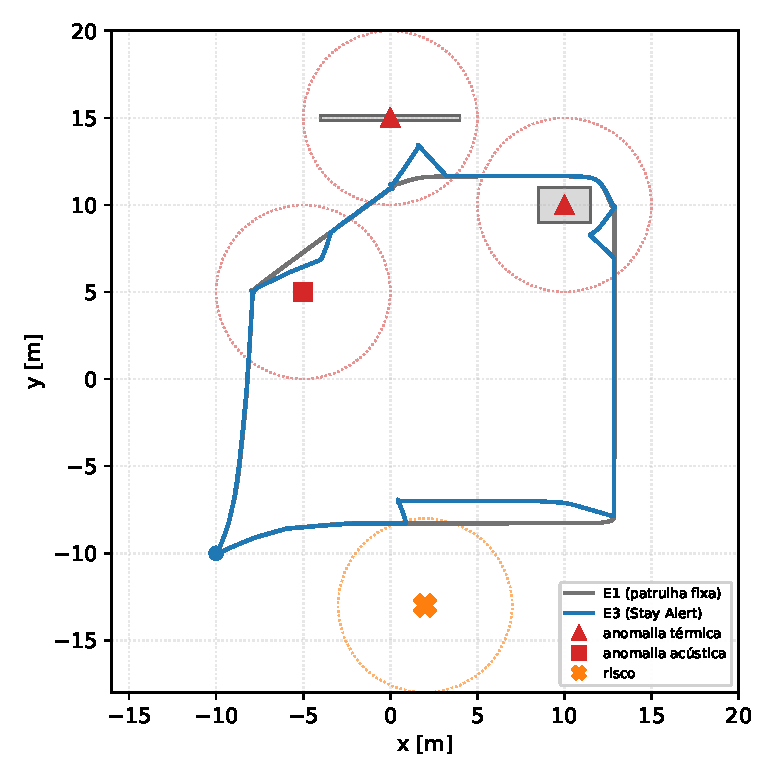
\includegraphics[width=0.85\textwidth]{figuras/traj_overlay}
\caption{Sobreposição de trajetórias da patrulha fixa (E1) e da camada reativa (E3)
no cenário padrão. A camada reativa abandona a perna de patrulha para alcançar a
pose de parada de cada anomalia e retorna à ronda; a patrulha fixa percorre o
circuito sem desvio.}
\label{fig:res-traj}
\end{figure}

\begin{figure}[htb]
\centering
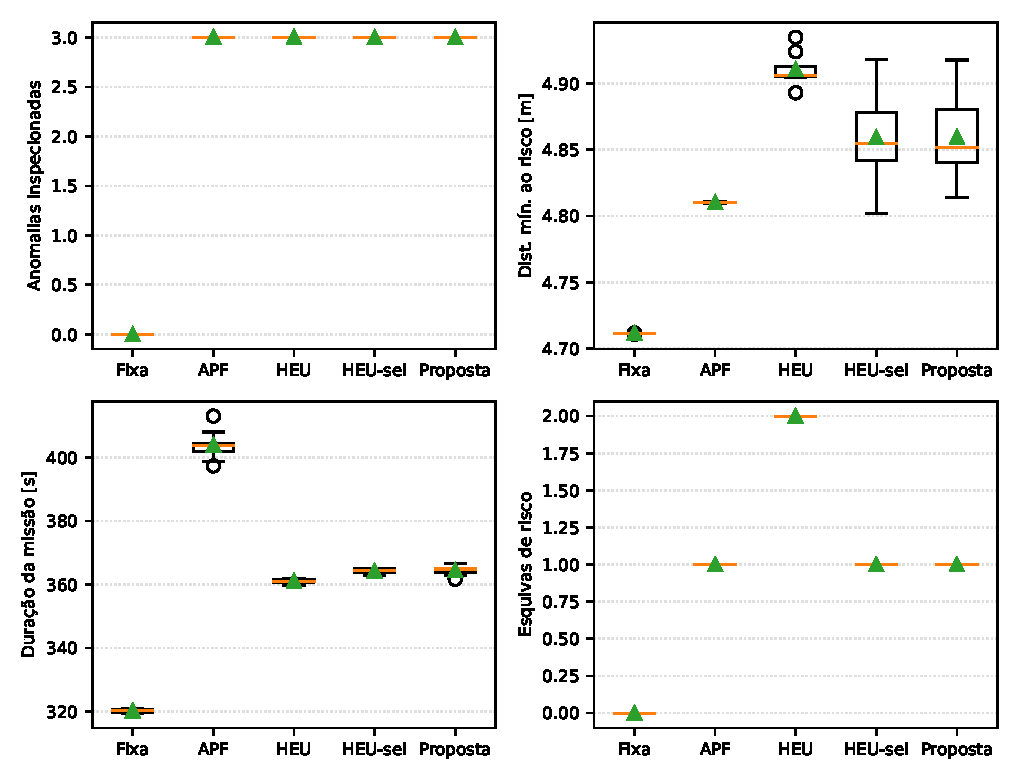
\includegraphics[width=0.95\textwidth]{figuras/box_panel}
\caption{Distribuições por execução das métricas principais ($\triangle$ = média),
todas no cenário \texttt{default}: a patrulha fixa, a linha de base de campo
potencial (APF), o supervisor heurístico genérico (HEU), a variante de seleção de um
fator (HEU-sel) e a camada proposta. A patrulha fixa nunca inspeciona nem recua; as
quatro configurações reativas inspecionam as três anomalias, e nenhuma diferença
estatisticamente detectável foi encontrada entre HEU-sel e a camada proposta em
qualquer das métricas exibidas. O HEU executa um segundo recuo e o APF precisa de
missão mais longa para as mesmas inspeções.}
\label{fig:res-box}
\end{figure}

\section{Isolando o Campo do Ato de Desviar}
\label{sec:res-heu}

As comparações da seção anterior contrastam a camada reativa com linhas de base que
ou não podem desviar (a patrulha fixa) ou alteram o controlador além do supervisor
(a linha de base de campo potencial). Nenhuma delas isola o \emph{campo} do ato de
desviar. Acrescentam-se, portanto, duas configurações que rodam sobre o \emph{mesmo}
controlador Nav2/MPPI, com a mesma percepção, o mesmo \textit{keep-out}, as mesmas
poses de aproximação, o mesmo critério de confirmação e a mesma lógica de retorno à
patrulha:

\begin{itemize}
    \item \textbf{HEU}, um supervisor genérico de
    detectar--selecionar--desviar--retornar: é acionado por \emph{detecção bruta}
    (um evento dentro do raio de sensoriamento) em vez de por limiar sobre $\Phi$,
    seleciona o alvo \emph{mais próximo} em vez do mais saliente, e arbitra pela
    regra simples ``risco no alcance $\Rightarrow$ desviar''. Substitui, portanto,
    tanto a ponderação por saliência quanto a arbitragem baseada em campo por
    equivalentes de detecção bruta. Note-se que ele ainda resolve riscos primeiro
    --- a verificação de preempção precede a verificação de atração ---, de modo que
    o que lhe falta não é uma regra de precedência, mas a persistência temporal que
    o campo com decaimento fornece.
    \item \textbf{HEU-sel}, variante de um fator: idêntica à camada proposta
    \emph{exceto} por selecionar o alvo mais próximo em vez do mais saliente.
\end{itemize}

Mudar o alvo selecionado não altera $\Phi$ no instante do disparo: o simulador
publica a intensidade de todo evento no alcance e o campo retém o máximo, de modo que
o cruzamento do limiar é o mesmo nos dois modos. Muda, porém, qual anomalia é
comprometida, e uma anomalia comprometida deixa de alimentar o campo. O contraste é,
assim, de seleção no ponto de decisão \emph{com} efeito a jusante sobre a evolução
temporal de $\Phi$, e não um mero reordenamento de atendimento.

A Tabela~\ref{tab:res-heu} relata os três cenários.

\paragraph*{Comparação primária (corrigida por Holm), cenário \texttt{default}.}
O HEU-sel não apresentou diferença estatisticamente detectável em relação à camada
proposta em nenhum dos cinco desfechos relatados ($p_{\mathrm{Holm}}=1{,}0000$ em
todos; $|\delta|\le0{,}19$; todos os intervalos \textit{bootstrap} contêm zero).
Dois dos cinco --- anomalias inspecionadas e recuos --- são constantes e idênticos
nos dois braços, enquanto os outros três variam. Trata-se de ausência de diferença
detectada com $n=10$, e não de demonstração de equivalência. Em contraste, o HEU
difere em recuos ($1$ contra $2$, $p_{\mathrm{Holm}}=3{,}0\times10^{-4}$), tempo de
investigação ($35{,}1$ contra $41{,}2$~s, $p_{\mathrm{Holm}}=0{,}0027$) e duração da
missão ($p_{\mathrm{Holm}}=0{,}0052$). A diferença de afastamento nesse cenário não
sobrevive à correção ($p_{\mathrm{Holm}}=0{,}0511$) e corresponde a $6$~cm, lida
aqui como operacionalmente irrelevante e relatada como tal, não como vantagem.

\paragraph*{Exploratório, cenário \texttt{conflict}.}
Nesse cenário um risco é colocalizado com uma anomalia \emph{mais saliente}, de modo
que as duas regras discordam por construção. A diferença é grande e na direção que a
precedência \emph{persistente} da camada proposta visa evitar: o HEU também
preempta, mas não mantém o canal de risco aberto. O HEU inspeciona a anomalia
colocalizada (mediana $4$ de $4$ contra $3$ da camada proposta) e paga por isso: o
afastamento mínimo cai de $4{,}84$ para $2{,}23$~m ($\delta$ de Cliff $+1{,}00$,
separação completa; IC \textit{bootstrap} da diferença $[+2{,}60;+2{,}63]$~m;
$p<0{,}0001$), os recuos sobem de $1$ para $4$ conforme o supervisor oscila, a
duração da missão cresce cerca de $106$~s, e o tempo até inspecionar o alvo
prioritário atrasa cerca de $105$~s em ambas as modalidades ($345{,}0$ contra
$239{,}9$~s na térmica; $387{,}6$ contra $283{,}1$~s na acústica). Para o HEU-sel,
novamente, nenhuma diferença em relação à camada proposta foi detectada em qualquer
desfecho relatado.

\paragraph*{Exploratório, cenário \texttt{adverse}.}
As três configurações alcançaram mediana de cinco anomalias inspecionadas, com
contagens por execução entre quatro e cinco (proposta $9/10$ execuções com cinco,
HEU $10/10$, HEU-sel $8/10$). O HEU executa um recuo adicional e as diferenças de
afastamento são da ordem de centímetros.

\begin{table}[htb]
\centering
\caption{Camada proposta contra supervisor genérico de
detectar--selecionar--desviar--retornar (HEU) e contra variante de seleção de um
fator (HEU-sel), todos sobre o mesmo controlador Nav2/MPPI. Medianas sobre execuções
válidas. O bloco \texttt{default} pertence à família de comparação primária
(corrigida por Holm); os blocos \texttt{conflict} e \texttt{adverse} são
exploratórios e são relatados com $p$ não corrigido. $n$: \texttt{default}
$10/9/10$, \texttt{conflict} $10/9/10$, \texttt{adverse} $10/10/10$
(proposta/HEU/HEU-sel).}
\label{tab:res-heu}
\footnotesize
\setlength{\tabcolsep}{4pt}
\begin{tabular}{llccccc}
\hline
\textbf{Cenário} & \textbf{Métrica} & \textbf{Proposta} & \textbf{HEU} &
\textbf{HEU-sel} & \textbf{$\delta$ (vs.\ HEU)} & \textbf{$p$ (vs.\ HEU)}\\
\hline
\texttt{default} & Anomalias inspecionadas    & $3$     & $3$     & $3$     & $+0{,}00$ & $1{,}0000^{\dagger}$\\
                 & Recuos                     & $1$     & $2$     & $1$     & $-1{,}00$ & $3{,}0\times10^{-4\dagger}$\\
                 & Dist.\ mín.\ ao risco [m]  & $4{,}85$  & $4{,}91$  & $4{,}85$  & $-0{,}73$ & $0{,}0511^{\dagger}$\\
                 & Tempo de investigação [s]  & $35{,}1$  & $41{,}2$  & $35{,}3$  & $-1{,}00$ & $0{,}0027^{\dagger}$\\
\hline
\texttt{conflict} & Anomalias inspecionadas   & $3$     & $4$     & $3$     & $-0{,}67$ & $0{,}0160$\\
                 & Recuos                     & $1$     & $4$     & $1$     & $-1{,}00$ & $0{,}0003$\\
                 & \textbf{Dist.\ mín.\ risco [m]} & $\mathbf{4{,}84}$ & $\mathbf{2{,}23}$ & $4{,}82$ & $+1{,}00$ & $<\!0{,}0001$\\
                 & Duração da missão [s]      & $363{,}7$ & $469{,}7$ & $364{,}4$ & $-0{,}89$ & $0{,}0013$\\
                 & Tempo até alvo prioritário [s]& $239{,}9$ & $345{,}0$ & $240{,}4$ & ---     & ---\\
\hline
\texttt{adverse} & Anomalias inspecionadas    & $5$     & $5$     & $5$     & $-0{,}10$ & $0{,}7337$\\
                 & Recuos                     & $1$     & $2$     & $1$     & $-1{,}00$ & $0{,}0002$\\
                 & Dist.\ mín.\ ao risco [m]  & $4{,}88$  & $4{,}90$  & $4{,}85$  & $-0{,}58$ & $0{,}0288$\\
\hline
\end{tabular}

\vspace{2pt}
\footnotesize $^{\dagger}$Corrigido por Holm dentro da família primária de $15$
testes. Linhas sem o símbolo são exploratórias e não corrigidas.
\end{table}

\subsection{O Que Se Pode e o Que Não Se Pode Atribuir}

Duas leituras decorrem desses números, e convém limitar cada uma.

Primeiro, o critério de \emph{seleção} não teve efeito detectável: nos cenários
\texttt{default} e \texttt{conflict} a camada proposta e o HEU-sel produziram o mesmo
valor constante em todo desfecho discreto ao longo das dez execuções de cada, e em
\texttt{adverse} os desfechos variam dentro dos dois grupos e se sobrepõem. Não se
alega equivalência --- com dez execuções por grupo, a falha em detectar uma diferença
não estabelece sua ausência, e não foram especificadas margens de equivalência para
essas métricas ---, apenas que o critério não fez diferença que aqui se pudesse
detectar.

Segundo, o efeito no cenário de conflito se prende ao \emph{modo de disparo}, por ser
este o único fator que separa HEU de HEU-sel. É preciso ser explícito quanto ao que
essa chave agrupa: ela substitui um limiar sobre o campo com decaimento por detecção
bruta instantânea, mudando o disparo \emph{e} removendo da decisão a persistência
temporal do campo. Ela \emph{não} remove a precedência de segurança. Os \textit{logs}
mostram o HEU preemptando a investigação três vezes por execução
(\texttt{deferred\_hazard}); cada adiamento libera o alvo, a atração volta a disparar
assim que o risco sai momentaneamente do alcance, e a inspeção acaba por se completar
--- o que é a oscilação visível como quatro recuos. Lê-se o efeito, portanto, como
perda de \emph{persistência temporal} no canal de risco, e não como ausência de regra
de precedência; apresenta-se essa como a leitura mais consistente com os
\textit{logs}, e não como fator isolado: separar a fonte do disparo da persistência
exigiria uma variante adicional que não foi executada.

\section{Resposta a Risco e Segurança}
\label{sec:res-seguranca}

A linha de base fixa registra zero esquivas de risco, enquanto a camada reativa
executa exatamente um recuo por encontro ($1{,}0\pm0{,}0$).

\subsection{Risco ao Lado da Rota}

Para o risco posicionado \emph{ao lado} da rota (E0--E5), o afastamento mínimo é
pequeno em termos absolutos para ambos, mas a camada reativa mantém afastamento
ligeiramente \emph{maior} e altamente consistente (E3, $4{,}86\pm0{,}03$~m) que a
linha de base fixa ($4{,}71\pm0{,}00$~m): a repulsão regula a aproximação a uma faixa
estreita, e a linha de base --- uma vez separadas as execuções com falha de partida
--- passa pelo risco lateral a uma distância fixa e marginalmente menor.

\subsection{Risco Sobre a Rota}

O teste mais informativo coloca o risco \emph{sobre} uma perna da patrulha
(configurações RHM, o método, e RHB, a linha de base fixa). Ali, a linha de base fixa
atravessa em linha reta, atingindo afastamento mínimo de apenas $0{,}71\pm0{,}00$~m
sem qualquer recuo e com tempo mínimo até a colisão de $2{,}8\pm0{,}1$~s. A camada
reativa produz resposta em duas escalas de tempo: tão logo o risco é detectado, ele é
projetado como zona de exclusão persistente no \textit{costmap} global --- de modo
que o planejador contorna pelo resto da missão --- e um recuo reativo rápido
($1{,}0\pm0{,}0$ evento de esquiva) trata a proximidade imediata. Os dois em conjunto
permitem ao robô contornar o risco a $1{,}71\pm0{,}01$~m (zero colisões nas execuções
válidas) com margem de tempo até a colisão de $5{,}6\pm0{,}9$~s, ainda inspecionando
todas as três anomalias ($3{,}0\pm0{,}0$), ao custo de tempo de $372\pm1$~s
(Tabela~\ref{tab:res-seguranca}).

A camada reativa, portanto, mais do que dobra o afastamento ($+1{,}00$~m; $\delta$ de
Cliff igual a $1$, $p<10^{-4}$) e aproximadamente dobra a margem de tempo até a
colisão ($+2{,}8$~s; $p<10^{-4}$) da patrulha fixa no caso que a repulsão existe para
tratar.

\begin{table}[htb]
\centering
\caption{Risco sobre a rota: desfechos de segurança (média\,$\pm$\,desvio padrão
sobre execuções válidas). RHB é a linha de base fixa (atravessa em linha reta); RHM é
o método --- recuo reativo combinado a zona de exclusão persistente disparada por
detecção, que o planejador contorna. $n$ válido: RHB $10$, RHM $9$.}
\label{tab:res-seguranca}
\footnotesize
\begin{tabular}{lcc}
\hline
\textbf{Métrica} & \textbf{RHB (base)} & \textbf{RHM (método)}\\
\hline
Anomalias inspecionadas        & $0{,}0\pm0{,}0$   & $3{,}0\pm0{,}0$\\
Recuos                         & $0{,}0\pm0{,}0$   & $1{,}0\pm0{,}0$\\
Colisões                       & $0{,}0\pm0{,}0$   & $0{,}0\pm0{,}0$\\
Dist.\ mín.\ ao risco [m]      & $0{,}71\pm0{,}00$ & $1{,}71\pm0{,}01$\\
Tempo mín.\ até colisão [s]    & $2{,}8\pm0{,}1$   & $5{,}6\pm0{,}9$\\
Tempo abaixo do afastamento [s]& $14{,}4\pm0{,}0$  & $9{,}2\pm0{,}1$\\
Duração da missão [s]          & $320\pm1$         & $372\pm1$\\
\hline
\end{tabular}
\end{table}

\subsection{A Quem Atribuir o Ganho de Segurança}
\label{sec:res-ablacao}

Para atribuir esse ganho a seus dois mecanismos, ablacionam-se ambos
(Tabela~\ref{tab:res-ablacao}). Com a \emph{zona de exclusão apenas} (KOa, recuo
reativo desabilitado) o planejador ainda contorna o risco e inspeciona as três
anomalias no mesmo afastamento de $1{,}71$~m, ligeiramente mais rápido que o método
completo ($352$ contra $372$~s). Com o \emph{recuo reativo apenas} (KOb, zona de
exclusão desabilitada) o robô não consegue livrar o risco sobre a rota: oscila
($29{,}6\pm3{,}9$ recuos), quase nada inspeciona ($0{,}2\pm0{,}4$) e estoura o tempo
($627\pm6$~s).

Essas duas ablações, porém, ainda carregam a camada reativa. A referência mais justa
é uma \emph{patrulha fixa portando a mesma zona de exclusão disparada por detecção e
nenhuma camada reativa}, que isola o \textit{keep-out} da ponderação; acrescenta-se,
portanto, a configuração KOF (camada reativa desabilitada, \textit{keep-out} ativo).
O KOF atinge afastamento mínimo mediano de $1{,}73$~m contra $1{,}71$~m da ablação
somente-\textit{keep-out} KOa --- diferença de $2$~cm que não é distinguível
($p_{\mathrm{Holm}}=0{,}4194$) --- e passa $9{,}0$~s abaixo da faixa de $2$~m contra
$9{,}3$~s.

\textbf{Atribui-se, portanto, o benefício de segurança sobre um risco na rota à zona
de exclusão disparada por detecção, e não à ponderação reativa.} O KOF não é cego ao
risco: ele percebe o risco e projeta a zona de exclusão; o que lhe falta é o
supervisor reativo.

O que a camada reativa acrescenta sobre o KOF é o comportamento de inspeção, e apenas
isso: o KOF inspeciona $0$ das $3$ anomalias em toda execução --- por construção,
pois sem camada reativa nenhuma investigação é jamais disparada --- contra $3$ de $3$
do KOa ($p_{\mathrm{Holm}}=1{,}6\times10^{-4}$), e completa a missão $31$~s mais
rápido ($320{,}9$ contra $352{,}2$~s, $p_{\mathrm{Holm}}=0{,}0021$) precisamente
porque nunca se desvia. O par KOF/KOa é, assim, uma decomposição e não uma vitória: a
zona de exclusão compra o afastamento, a camada reativa compra as inspeções, e as
duas coisas são separáveis.

A zona de exclusão deliberativa é, portanto, o mecanismo que resolve um risco sobre a
rota; o recuo reativo não acrescenta benefício mensurável para esse risco
\emph{estático}. Não se alega que o recuo ajude aqui --- seu valor aparece quando um
risco \emph{emerge} durante uma investigação, o que se quantifica a seguir.

\begin{table}[htb]
\centering
\caption{Ablação de zona de exclusão e recuo no risco sobre a rota
(média\,$\pm$\,desvio padrão sobre execuções válidas; $n=9$ para RHM, $10$ para KOa,
$9$ para KOb). RHM é o método completo (recuo $+$ zona de exclusão); KOa é
somente-zona (recuo desabilitado); KOb é somente-recuo (zona desabilitada).}
\label{tab:res-ablacao}
\footnotesize
\setlength{\tabcolsep}{5pt}
\begin{tabular}{lccc}
\hline
\textbf{Métrica} & \textbf{RHM} & \textbf{KOa} & \textbf{KOb}\\
 & \textbf{(recuo+zona)} & \textbf{(zona)} & \textbf{(recuo)}\\
\hline
Anomalias inspecionadas     & $3{,}0\pm0{,}0$   & $3{,}0\pm0{,}0$   & $0{,}2\pm0{,}4$\\
Recuos                      & $1{,}0\pm0{,}0$   & $0{,}0\pm0{,}0$   & $29{,}6\pm3{,}9$\\
Colisões                    & $0{,}0\pm0{,}0$   & $0{,}0\pm0{,}0$   & $0{,}0\pm0{,}0$\\
Dist.\ mín.\ ao risco [m]   & $1{,}71\pm0{,}01$ & $1{,}71\pm0{,}01$ & $4{,}29\pm0{,}08$\\
Tempo mín.\ até colisão [s] & $5{,}6\pm0{,}9$   & $5{,}8\pm0{,}1$   & $8{,}7\pm0{,}2$\\
Duração da missão [s]       & $372\pm1$         & $352\pm1$         & $627\pm6$\\
\hline
\end{tabular}
\end{table}

\section{O Valor do Recuo Diante de Risco Emergente}
\label{sec:res-emergente}

A ablação anterior mostra que, para um risco \emph{estático} sobre a rota, a zona de
exclusão deliberativa sozinha (KOa) iguala o método completo e o recuo reativo não
acrescenta benefício mensurável. O recuo foi projetado, contudo, para um risco que
\emph{emerge} enquanto o robô já está comprometido com uma inspeção --- o caso para o
qual a preempção do Algoritmo~\ref{alg:stayalert} foi construída e que os cenários
estáticos não conseguem exercitar.

Testa-se isso diretamente (configurações DHa, DHb): um risco colocalizado com uma
anomalia permanece inativo --- não publicado nem ao canal reativo nem à zona de
exclusão deliberativa --- até que o robô, já investigando, se aproxime a $3$~m, ponto
em que o ambiente o ativa. O instante de ativação e a primeira publicação em cada
canal são registrados por execução.

Os valores de afastamento e de tempo radial até a colisão abaixo são mínimos
\emph{de missão inteira} relativos à localização do risco, incluindo o período
anterior à ativação: o coletor não reinicia essas métricas na ativação. Esses
resultados comparam, portanto, margens de nível de missão no cenário de risco
emergente, e não estimam efeito de TTC pós-ativação separado. O tempo de simulação
preservado na auditoria permite localizar o mínimo de \emph{distância}: ele é
atingido após a ativação em todas as $18$ execuções dinâmicas válidas. Não se estende
isso ao mínimo de TTC --- que, sendo uma razão envolvendo velocidade radial, pode já
carregar valor anterior à ativação ---, de modo que a diferença de TTC é relatada
estritamente como margem de missão inteira.

Com o recuo reativo ativo (DHa) a preempção dispara em \emph{toda execução válida}
($8/8$ investigações adiadas) e o robô se afasta, mantendo afastamento mínimo de
$2{,}55\pm0{,}15$~m e tempo radial até a colisão de $5{,}23\pm0{,}45$~s. Com o recuo
desabilitado (DHb, somente zona de exclusão) o robô prossegue até a pose de parada da
inspeção, aproximando-se a $2{,}22\pm0{,}01$~m ($4{,}72\pm0{,}21$~s).

O recuo reativo compra, portanto, $+0{,}33$~m de afastamento (IC $95\%$
$[+0{,}23;+0{,}42]$, $\delta$ de Cliff igual a $1$, $p=4{,}6\times10^{-5}$) e
$+0{,}51$~s de margem de tempo até a colisão ($[+0{,}20;+0{,}84]$, $\delta=0{,}85$,
$p=1{,}0\times10^{-3}$) contra um risco emergente.

Essa margem é uma troca deliberada, não um ganho gratuito: DHa roda cerca de
$9{,}4$~s a mais ($348$ contra $338$~s) e $1{,}6$~m a mais, e \emph{adia} a inspeção
agora arriscada (DHa não inspeciona o alvo em execução alguma; DHb o inspeciona em
todas), comprando margem de segurança maior naquele encontro ao preço de uma inspeção
completada. Nenhuma das configurações entra na região de contato, e nenhuma passa
tempo algum abaixo do limiar de afastamento de $2$~m, de modo que o efeito é
diferença de \emph{margem}, não de contatos observados.

Distingue-se ainda o disparo da preempção de um recuo limpamente completado: em $3$
das $8$ execuções válidas de DHa, a meta de navegação do recuo é ela própria
abortada, e ainda assim cada episódio termina como esquiva bem-sucedida --- o campo
decai abaixo do limiar uma vez que o risco é entregue à zona de exclusão (saída
\emph{segura}) --- e o afastamento relatado é o mínimo de \emph{posição verdadeira}
do coletor de métricas, não uma chegada presumida à pose de recuo (essas três
execuções mantêm, de fato, $2{,}70$~m). A contribuição do recuo é, assim, uma margem
de segurança \emph{transiente} quando um risco aparece no meio da investigação ---
benefício que a ablação estática sobre a rota, por construção, não pode revelar.

\section{Precedência de Segurança sob Conflito}
\label{sec:res-conflito}

Os cenários precedentes separam atração e repulsão no espaço, de modo que o campo
nunca precisa arbitrar entre uma anomalia e um risco no mesmo local. O cenário de
conflito (CONF) força exatamente essa decisão: uma anomalia acústica \emph{forte}
($|w\,I_e|=1{,}14$) é colocalizada com um risco \emph{mais fraco}
($|w\,I_e|=1{,}05$) em $(2,-13)$, de sorte que uma regra de seleção puramente por
magnitude --- que retém o sinal mais saliente --- preferiria inspecionar a anomalia e
jamais disparar um recuo. A regra de precedência resolve primeiro qualquer risco
acima do limiar, independentemente de uma atração concorrente mais forte.

Trata-se de propriedade categórica de \emph{seleção}, não de efeito médio, e por isso
é relatada como frequência de desfecho e não como comparação de médias. Nas dez
execuções de CONF (todas válidas), o comportamento foi idêntico em todas:
\textsc{Avoid} foi disparado ($10/10$ execuções, $1{,}0\pm0{,}0$ recuos) e a anomalia
forte colocalizada \emph{nunca} foi inspecionada, de modo que o robô inspecionou
apenas as três anomalias fora do conflito ($3{,}0\pm0{,}0$). O robô manteve
afastamento mínimo ao risco de $4{,}84\pm0{,}02$~m e tempo mínimo até a colisão de
$17{,}3\pm1{,}6$~s, com \emph{zero} colisões em todas as execuções, a uma duração de
missão ($364\pm2$~s) indistinguível da do cenário padrão.

O campo reativo impõe, portanto, uma \emph{prioridade de seleção com risco em
primeiro lugar} por construção, confirmada empiricamente no único caso projetado para
quebrar uma interpretação puramente de magnitude. Essa é uma escolha deliberada de
projeto --- a prioridade é \emph{rígida}, de modo que um risco pouco acima do limiar
(um possível falso positivo) suprime mesmo uma anomalia genuína fortemente saliente
--- e aceita-se o risco resultante de excesso de conservadorismo. Distingue-se essa
prioridade \emph{lógica} de uma garantia física de segurança: ela vale sob condições
explícitas (uma pose de recuo disponível e fora da janela refratária pós-recuo), e o
cenário estático CONF não exercita casos como o de um segundo risco surgindo durante
a janela refratária. O que se relata como desfecho de \emph{segurança} é o
afastamento observado e a ausência de entradas na região de contato, não uma garantia
de invariância.

\section{O Custo da Precedência e Sua Sensibilidade}
\label{sec:res-custo-precedencia}

A seção anterior aceita um risco de excesso de conservadorismo próximo ao limiar sem
medi-lo. Mede-se agora, e sonda-se separadamente se o limiar que governa a
precedência está bem posicionado. Ambas as análises são exploratórias.

\subsection{Um Risco Marginalmente Elegível Custa Uma Inspeção, Deterministicamente}

O canal de risco tem memória: uma observação eleva $h$, e $h$ decai então por
$\lambda$ a cada período até cair abaixo de $\varepsilon$. Como o limiar de
modalidade é aplicado à intensidade bruta percebida, o risco elegível \emph{mais
fraco} já produz $h=|w_{\mathcal{H}}|\,\theta_{\mathcal{H}}$, que aqui iguala o
limiar de entrada do supervisor; um recuo dispara, portanto, uma vez, no pico. Após
um único passo de decaimento, porém, $h$ está abaixo do limiar de entrada enquanto
ainda acima de $\varepsilon$ --- de modo que o risco continua \emph{governando} o
campo, e assim continua suprimindo qualquer atração, sem disparar recuo adicional.

Construiu-se a configuração CM para exercitar exatamente essa faixa: um risco de
intensidade elegível mínima ao lado da primeira perna de patrulha, que o robô observa
e então deixa para trás, junto a uma anomalia acústica legítima de intensidade
$0{,}95$ --- o evento mais saliente do cenário --- posicionada a $4{,}3$~m do risco,
bem fora dele.

O resultado é o mesmo nas dez execuções: exatamente um recuo dispara e a anomalia
saliente \emph{nunca} é inspecionada ($0/10$), de modo que o robô encerra toda missão
tendo inspecionado $3$ das $4$ anomalias, abrindo mão da mais forte. Define-se a
janela de supressão como o intervalo entre a primeira e a última amostra registrada
em que o canal de risco governa o campo ($\Phi<0$) enquanto sua magnitude está abaixo
do limiar de recuo. Assim medida, ela dura $69{,}5$~s (faixa $67{,}3$--$72{,}4$). Não
é puro decaimento: o risco é reobservado dentro da janela e a magnitude do campo
volta a subir em uma mediana de duas amostras por execução, razão pela qual ela
excede os cerca de $39$~s que o decaimento sozinho, a partir da magnitude inicial,
daria.

A precedência categórica, portanto, não apenas arrisca excesso de conservadorismo:
nessa configuração ela custa uma inspeção em toda execução. O custo é incorrido sob
condições em que a própria camada não agiria sobre o risco --- ao longo de toda a
janela a distância mínima do robô a ele é de $3{,}92$~m (faixa $3{,}86$--$4{,}06$) e
sua magnitude está abaixo do limiar de recuo.

Enfatiza-se uma leitura que os números \emph{não} sustentam. CM e o cenário de
conflito completo terminam ambos com três anomalias inspecionadas, mas os dois trêses
não são comparáveis: em CONF a anomalia preterida é colocalizada com o risco e
\emph{deve} ser recusada, ao passo que em CM ela é alvo legítimo a $4{,}3$~m de
distância. A mesma contagem é comportamento correto em um cenário e falha no outro.

\subsection{Sensibilidade Local ao Limiar de Elegibilidade do Risco}

Variar o limiar de entrada do supervisor não testa a precedência, porque o que
governa a supressão é o limiar de \emph{elegibilidade de modalidade}
$\theta_{\mathcal{H}}$, aplicado antes da ponderação. Varre-se esse limiar sobre
$\{0{,}20;\,0{,}30;\,0{,}40\}$ no cenário de conflito, com $0{,}30$ o valor usado ao
longo de todo o trabalho.

Baixá-lo para $0{,}20$ não produziu diferença estatisticamente detectável
(afastamento $4{,}85$ contra $4{,}83$~m, $p=0{,}39$; inspeções e recuos idênticos).
Elevá-lo para $0{,}40$ \emph{degrada} a segurança: o afastamento mínimo cai para
$3{,}78$~m ($\delta$ de Cliff $+1{,}00$, IC \textit{bootstrap} da diferença
$[+0{,}99;+1{,}10]$~m, $p<0{,}0001$) e a missão se alonga em $9{,}1$~s, porque limiar
de elegibilidade mais alto significa que o risco é reconhecido mais tarde e, portanto,
mais perto. Relatam-se esses dois contrastes sem inferir curva de resposta geral a
partir de três valores; o que eles estabelecem é que o afastamento relatado no
restante do trabalho não é produzido por um limiar escolhido abaixo do valor em que a
degradação aparece.

\subsection{Histerese: Sem Efeito Detectável da Largura Testada, mas a Posição Importa}

Comparam-se três pares de entrada/saída escolhidos de modo que posição e largura
variem independentemente: a referência $(0{,}45;\,0{,}25)$, de largura $0{,}20$; uma
faixa mais estreita $(0{,}45;\,0{,}35)$, de largura $0{,}10$ no mesmo ponto de
entrada; e uma faixa deslocada $(0{,}55;\,0{,}35)$, de mesma largura $0{,}20$.

Reduzir a largura à metade não produziu diferença estatisticamente detectável em
qualquer desfecho relatado: desvios de rota, inspeções, duração da missão e tempo de
investigação dão todos $p\ge0{,}60$ contra a referência, com intervalos
\textit{bootstrap} contendo zero.

Deslocar o ponto de entrada dobra os desvios de rota contabilizados (mediana
$4\rightarrow8$, $\delta=-1{,}00$, $p=0{,}0003$) e reduz o tempo \emph{total} por
execução em \textsc{Investigate} (mediana $35{,}1\rightarrow26{,}6$~s, $p=0{,}0003$),
mantendo inalteradas as inspeções creditadas em $3$ de $3$. Mais desvios e menos
tempo total de investigação são, em conjunto, consistentes com o robô se comprometer
mais perto de cada alvo uma vez que o limiar de entrada é mais alto, mas os dois
agregados não separam duração de episódio de contagem de episódios, e não se
instrumentaram durações por episódio; oferece-se essa leitura como interpretação, e
não como medida. A métrica de desvios de rota deve ser lida como sensível à
\emph{posição} do limiar de entrada, e não como contagem intrínseca do cenário.

\section{Custo do Comportamento de Inspeção}
\label{sec:res-custo}

O comportamento acrescentado é barato: a duração de missão de E3 ($364\pm1$~s) é
aumento modesto sobre a linha de base fixa ($320\pm0$~s) pelos desvios de inspeção
($+6{,}2$~m percorridos). Enquadrado como troca de utilidade, cada anomalia adicional
inspecionada custa cerca de $2$~m de percurso extra ($+6{,}2$~m para três) e $15$~s
de tempo de missão ($+44$~s para três) --- troca favorável, dado que a linha de base
fixa não inspeciona \emph{nenhuma}.

\subsection{Lendo o Custo contra a Ronda}

Expresso contra a ronda que estende, o comportamento custa $14\%$ da duração da
patrulha: $320\pm0$~s tornam-se $364\pm1$~s por três inspeções. A maior parte desse
incremento é explicada pelo tempo total por execução em \textsc{Investigate} (mediana
$35{,}1$~s sobre os três episódios) e, como a permanência comandada é de apenas
$t_{\text{dwell}}=3$~s por episódio, o custo é dominado pelo desvio até a pose de
parada, e não pela pausa de inspeção em si.

Ele é também incorrido por \emph{evento}, e não por metro patrulhado, de modo que uma
ronda mais longa carregando o mesmo número de eventos distribuiria os mesmos segundos
absolutos sobre uma base maior e a penalidade relativa cairia. O cenário denso custa
mais em termos absolutos ($397\pm4$~s para $4{,}9\pm0{,}3$ inspeções) porque apresenta
mais eventos; seu \textit{layout} difere do padrão, de modo que não se lê a diferença
entre as duas rondas como incremento controlado.

A leitura prática para um operador é que cada inspeção creditada custa cerca de
$15$~s de tempo de ronda e cerca de $2$~m de percurso, e que uma ronda planejada com
essa folga para o número esperado de eventos absorve o comportamento sem
reprogramação da patrulha --- com a ressalva, da Seção~\ref{sec:res-ruido}, de que os
eventos precisam primeiro ser detectados.

\subsection{Comparação com a Linha de Base de Campo Potencial}

A camada proposta completa as mesmas três inspeções mais rápido ($364$ contra
$404\pm5$~s) sobre comprimento de caminho essencialmente igual ($86{,}6$ contra
$86{,}4$~m, diferença de $0{,}2$~m que não se lê como vantagem em direção alguma).

É preciso ser explícito quanto ao que essa comparação \emph{não} isola: a linha de
base APF substitui o supervisor reativo \emph{e} o controlador --- ela comanda
velocidades diretamente, em vez de emitir metas ao Nav2/MPPI ---, de modo que a
diferença confunde supervisor com controlador. Quanto ao ajuste, declaram-se
procedimento e valores. Os ganhos do APF foram calibrados para que a linha de base
dispare dentro do mesmo raio de sensoriamento da camada proposta --- atração cruzando
seu limiar em cerca de $4$ a $5$~m para \textit{waypoints} e repulsão na passagem a
cerca de $4{,}7$~m do risco lateral ---, critério de comparabilidade que foi o
aplicado. Os valores resultantes são $k_{\text{att}}=1{,}5$, $k_{\text{rep}}=4{,}0$,
$k_{\text{obs}}=0{,}6$, limiares de disparo e de saída de $0{,}15$ e $0{,}08$ sobre a
magnitude da força, e período refratário pós-recuo de $12$~s, acrescentado contra a
oscilação que a formulação de campo potencial exibe quando uma perna de patrulha
passa dentro da região de disparo. Além da calibração de alcance de disparo não se
buscou mais sobre esses valores, e a vantagem de tempo deve ser lida com isso em
mente. A comparação que \emph{de fato} isola o supervisor, sobre controlador e
parâmetros compartilhados, é a heurística da Seção~\ref{sec:res-heu}.

\section{Cenário Adverso}
\label{sec:res-adverso}

No cenário denso em eventos (E5) o robô arbitra entre eventos aglomerados pela regra
de precedência, inspecionando em média $4{,}9\pm0{,}3$ das cinco anomalias, com
desvios correspondentemente mais numerosos ($9{,}4\pm0{,}8$) e missão mais longa
($397\pm4$~s). A inspeção completa das cinco é bem-sucedida em $9$ de $10$ execuções
(intervalo de Wilson de $95\%$ $[0{,}60;\,0{,}98]$).

A trilha de auditoria por episódio mostra a causa com precisão: todos os cinco alvos
são \emph{iniciados} em toda execução, e a incompletude é falha de navegação, não
falha em revisitar. Três execuções registraram falha de navegação reativa; duas delas
subsequentemente \emph{iniciaram uma investigação adicional} e completaram os cinco
alvos, enquanto a execução restante terminou com quatro inspeções creditadas e
\emph{nenhuma nova tentativa registrada} sobre o alvo falho. As duas investigações
adicionais são relatadas como observação dos episódios, não como demonstração de
política de nova tentativa: o ramo \texttt{failed} marca o alvo como falho mas não o
remove do conjunto comprometido, de modo que um início posterior é possível, mas não
garantido por regra explícita de recuperação.

Esse limite de densidade --- a navegação reativa ocasionalmente falhando sobre um
alvo densamente aglomerado --- é medido, e não suposto inexistente, sem entradas na
região de contato observadas. Não se alega escalabilidade geral a partir de uma única
configuração adversa, e varreduras mais amplas de densidade e geometria permanecem
trabalho futuro.

\section{Robustez a Ruído de Percepção}
\label{sec:res-ruido}

Como a abstração de eventos fornece modalidade, intensidade e posição sem incerteza,
sonda-se a sensibilidade do método a essa idealização injetando ruído gaussiano de
média zero sobre a posição e a intensidade percebidas do evento a cada ciclo de
sensoriamento.

Sob ruído moderado (posição $\sigma=0{,}3$~m, intensidade $\sigma=0{,}05$;
configuração N1) o método não é afetado: inspeciona todas as três anomalias em toda
execução válida ($3{,}0\pm0{,}0$), com a resposta a risco preservada e sem colisões.

Sob ruído alto ($\sigma=0{,}6$~m, $\sigma=0{,}10$; N2), a completude de inspeção se
degrada para $4/9$ inspeções completas, e os \textit{logs} permitem atribuir a causa
com precisão: as três anomalias ainda são \emph{detectadas} em toda execução, mas a
estimativa ruidosa de posição conduz o robô a um ponto a partir do qual o avaliador
não consegue confirmar a chegada à anomalia \emph{verdadeira}, de modo que $6$ das
$27$ inspeções comprometidas (ao longo das $9$ execuções válidas) são
\emph{rejeições na confirmação} --- e não esgotamentos de tempo ou abortos de
navegação, dos quais os arquivos CSV não registram nenhum. A inspeção completa
sucede, portanto, em $4$ de $9$ execuções válidas ($2{,}3\pm0{,}7$ anomalias;
intervalo de Wilson de $95\%$ $[0{,}19;\,0{,}73]$ para a taxa de conclusão por
missão).

Nenhuma entrada na região de contato foi observada, e o recuo diante do risco foi
preservado ($1{,}7\pm0{,}5$; Tabela~\ref{tab:res-ruido}); o afastamento mínimo médio
ao risco de fato \emph{aumentou}, de $4{,}86\pm0{,}03$~m em E3 para
$5{,}29\pm0{,}20$~m em N2. Esses resultados descrevem a troca observada sob os níveis
de ruído testados --- a completude de inspeção cai, pela etapa de confirmação,
enquanto nenhum contato é observado e o afastamento medido cresce --- e não
estabelecem garantia geral de segurança.

\begin{table}[htb]
\centering
\caption{Robustez a ruído de percepção (método, média\,$\pm$\,desvio padrão). E3 é
sem ruído; N1 e N2 adicionam ruído gaussiano de média zero, moderado e alto, sobre
posição ($\sigma_p$) e intensidade ($\sigma_i$) do evento. ``Taxa de inspeção
completa'' é a fração por missão de execuções que inspecionam todas as três
anomalias. $n$ válido: E3 $10$, N1 $10$, N2 $9$.}
\label{tab:res-ruido}
\footnotesize
\begin{tabular}{lccc}
\hline
\textbf{Métrica} & \textbf{E3 (sem)} &
\textbf{N1 ($\sigma_p{=}0{,}3$)} & \textbf{N2 ($\sigma_p{=}0{,}6$)}\\
\hline
Anomalias inspecionadas    & $3{,}0\pm0{,}0$  & $3{,}0\pm0{,}0$  & $2{,}3\pm0{,}7$\\
Taxa de inspeção completa  & $10/10$          & $10/10$          & $4/9$\\
Recuos                     & $1{,}0\pm0{,}0$  & $1{,}1\pm0{,}3$  & $1{,}7\pm0{,}5$\\
Colisões                   & $0{,}0\pm0{,}0$  & $0{,}0\pm0{,}0$  & $0{,}0\pm0{,}0$\\
Dist.\ mín.\ ao risco [m]  & $4{,}86\pm0{,}03$& $5{,}01\pm0{,}11$& $5{,}29\pm0{,}20$\\
Duração da missão [s]      & $364\pm1$        & $367\pm5$        & $374\pm8$\\
\hline
\end{tabular}
\end{table}

\section{Ameaças à Validade}
\label{sec:res-ameacas}

Esta seção enumera o que a avaliação não estabelece.

\paragraph*{Percepção idealizada.} A percepção é abstraída em eventos-oráculo. A
Seção~\ref{sec:res-ruido} relaxa parcialmente essa idealização, mas falsos positivos,
falsos negativos, persistência de eventos e erro de localização permanecem fora do
estudo. A transformada de localização é fixa.

\paragraph*{Apenas simulação.} Todos os resultados vêm do Gazebo Fortress. Não há
validação em subestação física, e não se alega transferência direta para
\textit{hardware}.

\paragraph*{Tamanho amostral.} Com $8$ a $10$ execuções válidas por configuração, a
ausência de diferença detectada não demonstra equivalência, e a ausência observada de
entradas na região de contato limita, mas não elimina, o risco. O limite superior
unilateral exato de $95\%$ sobre a probabilidade por execução de tal entrada,
$1-0{,}05^{1/n}$, é de $25{,}9\%$ para um grupo de $10$ execuções, $28{,}3\%$ para um
grupo de $9$ e $31{,}2\%$ para o grupo de $8$ execuções de DHa. Esse limite de risco é
consequência do tamanho amostral, não medida de desempenho.

\paragraph*{Desfechos retrospectivos.} Como registrado na
Seção~\ref{sec:res-familias}, os três contrastes primários precedem os dados, mas o
conjunto de cinco desfechos foi fixado após as execuções. A correção de Holm trata a
multiplicidade dentro da família relatada; ela não torna prospectiva a seleção de
desfechos.

\paragraph*{Generalização de cenário.} Cada propriedade comportamental foi
estabelecida em uma configuração projetada para exercitá-la. Um único cenário adverso
não estabelece escalabilidade a \textit{layouts} mais densos, e um único cenário de
conflito não estabelece a precedência sob toda geometria de conflito.
